\documentclass[../main.tex]{subfiles}
\usepackage[utf8]{inputenc}
\usepackage[T1]{fontenc}
\usepackage{graphicx}
\usepackage{longtable}
\usepackage{wrapfig}
\usepackage{rotating}
\usepackage[normalem]{ulem}
\usepackage{amsmath}
\usepackage{amssymb}
\usepackage{capt-of}
\usepackage{hyperref}
\usepackage{float}
\graphicspath{{../}}
\author{Cezary Wieczorkowski}
\date{\today}
\title{Analiza}
\hypersetup{
 pdfauthor={Cezary Wieczorkowski},
 pdftitle={Analiza},
 pdfkeywords={},
 pdfsubject={},
 pdflang={Polish}}
\begin{document}


\section{Analiza istniejącego stanowiska}
Poniższy rozdział został napisany na podstawie \hyperref[zal:1]{załącznika nr 1}.   
\subsection{Zasada działania stanowiska}
    
    \subsubsection{Opis stanowiska}
        Zestaw laboratoryjny modeluje system komunikacji oparty na 4 bitowej szynie danych. W skład zestawu wchodzą urządzenia nadawcze i odbiorcze
        podłączone do szyny danych, logika sterująca procesem wymiany danych oraz elementy interfejsu użytkownika. Na rysunku \ref{fig:szyna_schemat} 
        można zobaczyć płytę czołową zestawu która przedstawia jego schemat blokowy oraz interfejs użytkownika. 
        \par
        W przypadku tego stanowiska działanie wspomnianych urządzeń jest emulowane na dwóch mikrokontrolerach. W dalszej części rozdziału
        działanie zestawu zostanie opisane tak jakby było to urządzenie zbudowane z podzespołów przedstawionych na jego płycie czołowej.

        \begin{figure}[H]
            \centering
            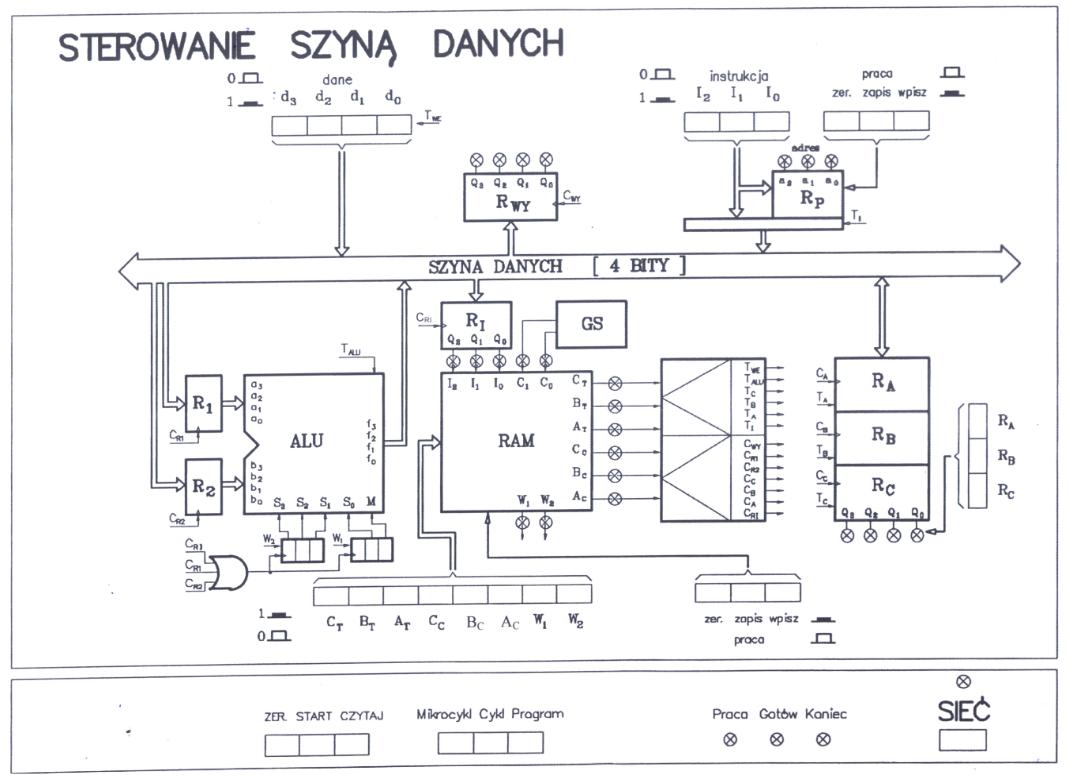
\includegraphics[width=\linewidth]{szyna_schemat.png}
            \caption{Płyta czołowa zestawu}
            \label{fig:szyna_schemat}
        \end{figure}

    \subsubsection{Elementy składowe stanowiska}

        \subsubsection*{Pamięć RAM}

        Pamięć ram w zestawie jest zorganizowana jako 32 słowa po 8 bitów.
        \begin{table}[ht]
            \centering
            \begin{tabular}{|ccc|ccc|cc|}
                \hline
                $C_T$ & $B_T$ & $A_T$ & $C_C$ & $B_C$ & $A_C$ & $W_1$ & $W_2$ \\ \hline
            \end{tabular}
            \caption{Symbole przypisane  poszczególnym bitom słowa w pamięci RAM}
            \label{tab:ram_symbol}
        \end{table}
        
        Zawartość słów w pamięci RAM kontroluję pracę zestawu:

        \begin{itemize}
            \item bity $C_T, B_T, A_T$ - wybór nadajnika na szynie
            \item bity $C_C, B_C, A_C$ - wybór odbiornika na szynie
            \item bity $W_1, W_2$ - wybór operacji ALU
        \end{itemize}

        Można zauważyć, że pamięć RAM zawiera instrukcje pracy zestawu. W celu wykonania kolejnych instrukcji należy zwiększyć o 1
        obecny adres pamięci. Wykonanie jednej instrukcji z pamięci RAM nazywamy mikrocyklem.
        \par
        Wejścia adresowe pamięci są połączone z rejestrem Rp (trzy najstarsze bity) oraz z generatorem Gs (dwa najmłodsze bity). 
        Trzy najstarsze bity wyjścia danych pamięci połączone są z wejściami adresowymi dekodera 1 natomiast kolejne trzy z wejściami 
        adresowymi dekodera 2. Dwa najmłodsze bity wyjścia danych pamięci połączone są wejściami informacyjnymi rejestrów przesuwnych instrukcji ALU.

        \subsubsection*{Generator GS}
        
        Generator GS jest licznikiem modulo 4. Jego wyjścia połączone są z dwoma najmłodszymi wejściami adresowymi pamięci RAM. Podczas pracy
        generator wygeneruje kolejno wartości dwóch najstarszych bitów adresu od 00 do 11. W zależności od trybu pracy zestawu generowane są
        kolejne adresy pamięci do zapisu lub odczytu i wykonani jako instrukcje w mikrocyklu.

        \subsubsection*{Dekoder sygnałów sterujących}
        
        Dekodery sygnałów sterujących to układy konwertujące liczby binarne na kod 1 z n. Dekoder 1 wytwarza sygnały sterujące nadajnikami które
        podawane są na wejścia sterujące przyłączaniem poszczególnych nadajników do szyny danych.

        \begin{table}[ht]
            \centering
            \[
            \begin{array}{|ccc|cccccc|}
            \hline
            C_T & B_T & A_T & T_I & T_A & T_B & T_C & T_{ALU} & T_{WE} \\ \hline
            0   & 0   & 0   & 1   & 0   & 0   & 0   & 0       & 0     \\ \hline
            0   & 0   & 1   & 0   & 1   & 0   & 0   & 0       & 0     \\ \hline
            0   & 1   & 0   & 0   & 0   & 1   & 0   & 0       & 0     \\ \hline
            0   & 1   & 1   & 0   & 0   & 0   & 1   & 0       & 0     \\ \hline
            1   & 0   & 0   & 0   & 0   & 0   & 0   & 1       & 0     \\ \hline
            1   & 0   & 1   & 0   & 0   & 0   & 0   & 0       & 1     \\ \hline
            \end{array}
            \]
            \caption{Tablica prawdy dla dekodera 1}
            \label{tab:nadajniki}
        \end{table}

        Dekoder 2 działa analogicznie do dekodera 1 ale wytwarza sygnały sterujące odbiornikami. Sygnały generowane przez dekoder 1 podawane
        są na wejścia zapisu poszczególnych odbiorników.

        \begin{table}[ht]
            \centering
            \[
            \begin{array}{|ccc|ccccccc|}
            \hline
            C_C & B_C & A_C & C_{RI} & C_A & C_B & C_C & C_{R1} & C_{R2} & C_{WY} \\ \hline
            0   & 0   & 0   & 1      & 0   & 0   & 0   & 0      & 0      & 0      \\ \hline
            0   & 0   & 1   & 0      & 1   & 0   & 0   & 0      & 0      & 0      \\ \hline
            0   & 1   & 0   & 0      & 0   & 1   & 0   & 0      & 0      & 0      \\ \hline
            0   & 1   & 1   & 0      & 0   & 0   & 1   & 0      & 0      & 0      \\ \hline
            1   & 0   & 0   & 0      & 0   & 0   & 0   & 1      & 0      & 0      \\ \hline
            1   & 0   & 1   & 0      & 0   & 0   & 0   & 0      & 1      & 0      \\ \hline
            1   & 1   & 0   & 0      & 0   & 0   & 0   & 0      & 0      & 1      \\ \hline
            \end{array}
            \]
            \caption{Tablica prawdy dla dekodera 2}
            \label{tab:odbiorniki}
        \end{table}

        \subsubsection*{Jednostka arytmetyczno logiczna ALU}
        
        Układ ten realizuje operacje arytmetyczne i logiczne na dwóch liczbach 4 bitowych zapisanych w rejestrach $R_1$ oraz $R_2$.
        Rodzaj wykonywanej operacji określa pięciobitowe słowo $M, S_3, S_2, S_1, S_0$ które jest zapisywane w dwóch 3 bitowych rejestrach przesuwnych.
        Na rysunku \ref{fig:szyna_schemat} pokazano sposób połączenia rejestrów przesuwnych w układzie. Na ich wejścia danych podane są 
        sygnały $W_1, W_2$ z pamięci RAM. Natomiast na wejścia zegarowe podana jest suma logiczna sygnałów $C_{RI}, C_{R1}, C_{R2}$. Z tych zależności
        wynika, że podczas projektowania instrukcji z użyciem ALU w celu ustawienia odpowiedniego kodu operacji należy przewidzieć 
        wygenerowanie sygnałów $C_{RI}, C_{R1}, C_{R2}$. Na rysunku \ref{fig:kodowanie_alu} przedstawiono sposób kodowania operacji do wykonania przez ALU.

        \begin{figure}[H]
            \centering
            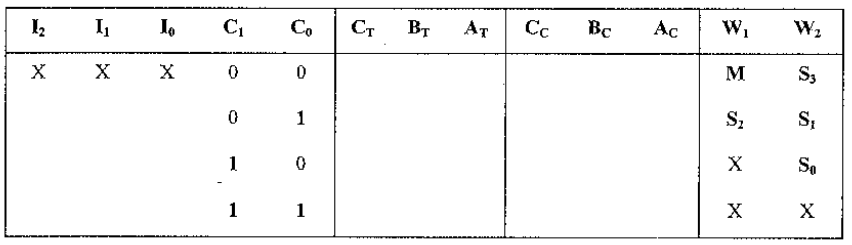
\includegraphics[width=\linewidth]{kodowanie_alu.png}
            \caption{Zasada kodowania operacji do wykonania przez ALU}
            \label{fig:kodowanie_alu}
        \end{figure}

        Jednostka arytmetyczno logiczna ma możliwość zrealizowania 16 operacji arytmetycznych oraz logicznych:

        \begin{figure}[H]
            \centering
            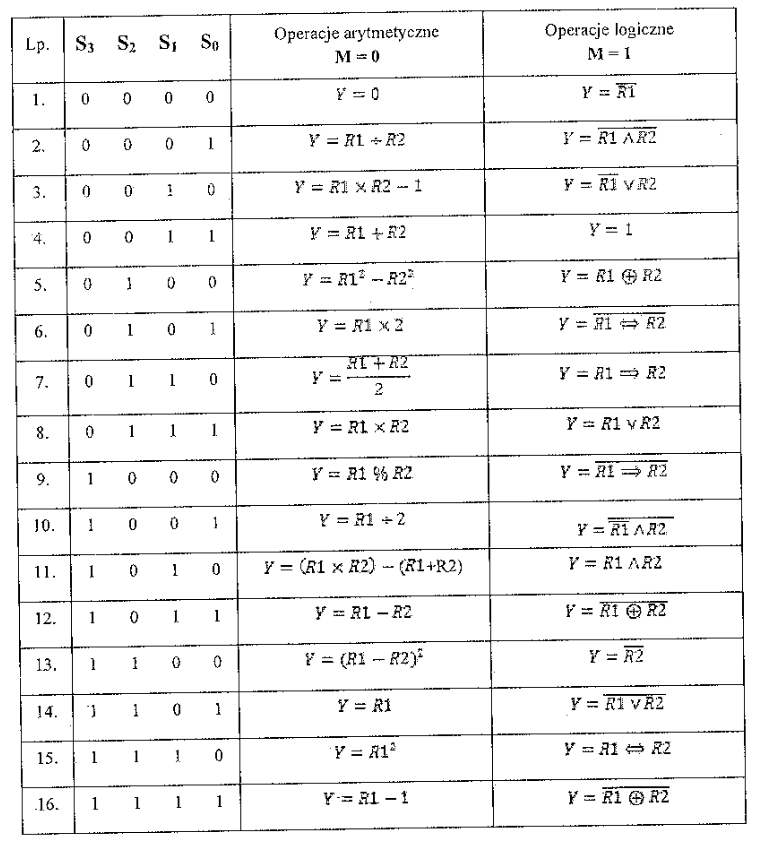
\includegraphics[width=\linewidth]{operacje_alu.png}
            \caption{Lista operacji realizowanych przez ALU}
            \label{fig:operacje_alu}
        \end{figure}

        \subsubsection*{Rejestry pomocnicze}
        Rejestry są układami przechowującymi dane. W zestawie występują następujące rejestry:
        \begin{itemize}
            \item $R_A, R_B, R_C$ - są to rejestry przeznaczone do wykorzystania przez użytkownika, 
            mogą one zarówno odbierać jak i nadawać dane na szynę
            \item $R_1, R_2$ - przechowują argumenty operacji ALU, mogą tylko odbierać dane z szyny
            \item $R_{wy}$ - służy do prezentacji wyników operacji wykonywanych przez zestaw laboratoryjny, może tylko odbierać dane z szyny
            \item $R_I$ - przechowuje trzy najstarsze bity adresu pamięci, może tylko odbierać dane z szyny
            \item $R_p$ - to zespół ośmiu rejestrów przeznaczonych do przechowywania adresów pamięci RAM pod którymi znajdują
            się instrukcje do wykonania przez zestaw. Rejestr ten jest wykorzystywany w trybie pracy Program
        \end{itemize}

    \subsubsection{Interfejs użytkownika}

    Na rysunku \ref{fig:szyna_schemat} poza schematem blokowym zestawu widzimy przyciski oraz diody LED służące do sterowania zestawem i 
    monitorowania jego pracy. 

    \subsubsection*{Kontrola pracy zestawu}
    Do sterowania pracą zestawu służą następujące przyciski:
    \begin{itemize}
        \item ZER. - przycisk zerowania generatora GS
        \item START - przycisk rozpoczynający pracę zestawu
        \item CZYTAJ - przycisk inicjujący odczyt z klawiatury dane i kontynuacje pracy zestawu
        \item Mikrocykl, Cykl, Program - przełączniki wyboru trybu pracy zestawu
        \item klawiatura dane - klawiatura do wprowadzania danych wejściowych na szynę danych
    \end{itemize}
    
    \subsubsection*{Zapis i odczyt danych z pamięci RAM}
    Do obsługi zapisu pamięci RAM służą przyciski:
    \begin{itemize}
        \item zer. - zerowanie adresu przy zapisie i odczycie pamięci RAM
        \item zapis/praca - wybór pomiędzy zapisem danych do pamięci RAM a pracą zestawu
        \item wpisz - zapis danych z klawiatury do RAM po jego wciśnięciu adres zwiększa się o 1
        \item klawiatura $C_T$ - $W_2$ - przyciski do ustawiania wartości bitowej słowa wpisywanego do pamięci RAM
    \end{itemize}

    \subsubsection*{Zapis i odczyt danych z $R_P$}
    Zapis oraz odczyt danych z rejestru odbywa się podobnie jak w przypadku pamięci RAM z użyciem odpowiednich przycisków:
    \begin{itemize}
        \item klawiatura dane - klawiatura do wprowadzania danych wejściowych na szynę danych
        \item klawiatura instrukcja - klawiatura do wprowadzania wartości do rejestru $R_P$
        \item zer. - zerowanie adresu przy zapisie i odczycie pamięci $R_P$
        \item zapis/praca - wybór pomiędzy zapisem danych do pamięci $R_P$ a pracą zestawu
        \item wpisz - zapis danych z klawiatury instrukcja do $R_P$ po jego wciśnięciu adres zwiększa się o 1
    \end{itemize}

    \subsubsection*{Monitorowanie pracy zestawu}
    Na płycie czołowej zestawu znajdują się również diody LED obrazujące wartości 

    \begin{itemize}
        \item Adresu pamięci RAM
        \item Wartości słowa w pamięci RAM
        \item Wartości słowa w rejestrze $R_{WY}$
        \item Wartości słowa w jednym z rejestrów $R_A, R_B, R_C$ wybieranych przyciskami
        \item Adres rejestru $R_P$
    \end{itemize}

    \subsubsection{Tryby pracy stanowiska}
    Stanowisko posiada trzy tryby pracy:
    \begin{itemize}
        \item  Mikrocykl - zestaw po wciśnięciu przycisku START wykona tylko jedną instrukcję z pamięci RAM, zostanie wygenerowana 
        tylko jedna wartość w generatorze GS. Po jej wykonaniu zestaw zatrzyma się i będzie oczekiwał na ponowne wciśnięcie przycisku START.
        \item  Cykl - zestaw po wciśnięciu przycisku START wykona cztery kolejne instrukcje z pamięci RAM. Nastąpią cztery kolejne zmiany
        wyjść w generatorze GS. Po wykonaniu czterech instrukcji zestaw zatrzyma się i będzie oczekiwał na ponowne wciśnięcie przycisku START.
        \item Program - po wciśnięciu przycisku START zestaw poda na wyjście rejestru $R_P$ kolejno osiem instrukcji które zostały
        do niego uprzednio zapisane. Układ wygeneruje kolejne 32 stany generatora GS, zmiana wartości w rejestrze $R_P$ nastąpi co czwartą
        wartość generatora GS.
    \end{itemize}

    Niezależnie od trybu pracy zestawu automatycznie generowane są tylko wartości generatora GS. W celu wykonania kolejnych instrukcji należy 
    manualnie załadować wartość trzech najstarszych bitów adresu pamięci kolejnej instrukcji do rejestru $R_I$. 
    W tym celu w pierwszej instrukcji każdego bloku czterech instrukcji w pamięci RAM należy umieścić wartość 000000XX. Taka wartość instrukcji 
    odpowiada ustawieniu rejestru $R_I$ jako odbiornika a rejestru $R_P$ jako nadajnika. W przypadku pracy w trybie Mikrocykl oraz Cykl wartość trzech
    najstarszych bitów adresu pamięci kolejnej instrukcji należy za każdym razem manualnie wprowadzić na klawiaturze instrukcji. Natomiast w trybie
    Program kolejne osiem wartości rejestru $R_P$ zostanie automatycznie podanych na jego wyjście.


\subsection{Krytyczna ocena stanowiska}

    \subsubsection{Założenia funkcjonalne}

    Zestaw w obecnej formie pozwala na realizacje prostych programów obrazujących działanie szyny danych w praktyce. Urządzenia podłączone do szyny
    współpracują ze sobą w sposób przemyślany pozwalają na realizowanie prostych operacji na jednostce ALU, zapis danych do rejestrów, pobieranie
    oraz prezentowanie danych użytkownikowi. Tryby pracy zestawu pozwalają na łatwe zaobserwowanie procesów zachodzących w zestawie podczas
    wykonywania programu. Tryby cykl i mikrocykl ułatwiają debugowanie programów przechodząc przez każdy cykl lub mikrocykl programu.

    \subsubsection{Interfejs użytkownika}

    Interfejs użytkownika zestawu opiera się na przyciskach jako urządzeniach wejściowych oraz diodach LED jako urządzeniach wyjściowych. Wizualizacja
    stanu poszczególnych rejestrów oraz bitów za pomocą diod LED jest czytelna i intuicyjna. W połączeniu ze schematem blokowym na płycie pozwala
    to w łatwy sposób zrozumieć jakie działania zestaw wykonuje w danym momencie. Możliwość podglądu adresu pamięci RAM oraz słowa 
    pod nim zapisanego ułatwia znajdywanie błędów w programach uruchamianych na zestawie.
    \par
    Wprowadzanie danych do zestawu (wartości pamięci RAM, rejestru $R_P$ oraz danych na szynę) odbywa się za pomocą klawiatur. Jest to kilka przycisków
    gdzie każdy przycisk odpowiada jednemu bitowi wprowadzanego słowa. Wciśnięty przycisk odpowiada wartości 1 a wyciśnięty wartości 0.
    Wprowadzanie wartości danych binarnych w ten sposób jest intuicyjne i szybkie.
    \par
    Pozostałe przyciski zestawu służą do kontroli jego pracy oraz kontroli procesów zapisu i odczytu wartości z pamięci RAM oraz rejestru $R_P$.
    Jest to sposób sprawdzony i stosunkowo intuicyjny. Głównym ograniczeniem tego podejścia jest trudność w dokonaniu zmian w interfejsie gdyż
    jego elementy są stałymi elementami płyty czołowej zestawu. Kolejnym ograniczeniem tego podejścia jest ograniczona możliwość sposobów zapisu oraz 
    odczytu pamięci RAM oraz rejestru $R_P$. Zapis oraz odczyt musi się odbywać w sposób sekwencyjny co znacząco wydłuża proces w przypadku gdy 
    zachodzi potrzeba zmiany lub odczytu wartości znajdujących się w dalszych regionach pamięci lub rejestru.

    \subsubsection{Platforma sprzętowa}

    W obecnej formie zestaw jest oparty o dwa mikrokontrolery Atmega 8 oraz Atmega 32. Odpowiadają one za symulację pracy komponentów składowych zestawu
    oraz obsługę interfejsu użytkownika. Emulacja komponentów zestawu programowo niesie za sobą szereg zalet: możliwość łatwej modyfikacji
    działania zestawu, mniejszy pobór mocy niż w przypadku dedykowanych układów scalonych. Podejście emulacyjne jest po części wymuszone 
    ograniczoną dostępnością w handlu dedykowanych układów scalonych takich jak jednostki ALU ze względu na ich znikomą popularność nowych projektach.
    \par
    Dużym problemem w przypadku tego zestawu jest to, że kod źródłowy programów pracujących na mikrokontrolerach w zestawie nie jest dostępny. 
    W przypadku potrzeby naprawy błędów w oprogramowaniu bądź chęci rozwinięcia funkcjonalności zestawu konieczne byłoby napisanie
    całego oprogramowania od nowa, co wiązałoby się z dużym nakładem pracy. Architektura oparta o dwa osobne układy na 
    których pracują różne programy również nie jest optymalna. Podział zadań na dwa mikrokontrolery komplikuje proces pisania oprogramowania oraz
    naprawy potencjalnych błędów.

\end{document}